В ходе вычислительных экспериментов выяснилось, что только четверть из всего набора признаков (см. раздел~\ref{features}) встречалась в данном наборе тестовых данных (см. раздел~\ref{test_data}). Остальные признаки отсутствовали, т.е. их значения для данной выборки были нулевыми. Поскольку алгоритм классификации Random Forest базируется на методе случайных подпространств (см. раздел~\ref{random_forest}), признаки, по которым строятся деревья решений для дальнейшей классификации, выбираются случайным образом. Как следствие, при выборе признаков из всего изначального их набора приводит к тому, что построение деревьев решений производится в преимущественной доли случаев на нулевых значениях признаков и приводит к существенному снижению точности классификации. Данная проблема была решена обрезанием статистически незначимых признаков на каждой новой итерации классификации.  

График, отображающий статистически значимые признаки для используемого набора данных можно увидеть на рисунке~\ref{important:important}.

\begin{figure}[h!]
\center{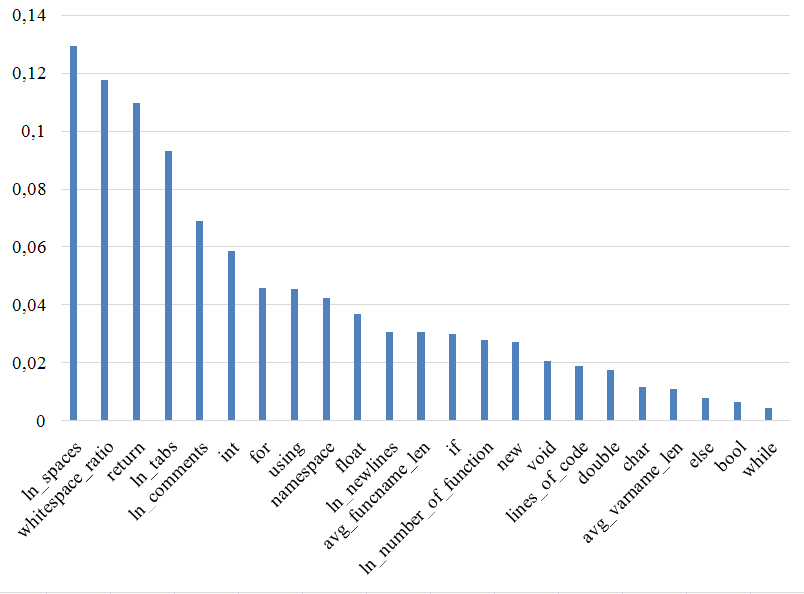
\includegraphics[width=0.9\linewidth]{important}}
\caption{ Статистически значимые признаки}
\label{important:important}
\end{figure} 
